\chapter{Results}\label{chap:results}
Only the test result from the Hardware-only test will be presented, to get an overview of the different simulation test see \cite{DavidThesis}. The analysis of the result will also be more qualitative than quantitative. For a more quantitative approach see \cite{DavidThesis}. For the PrintSat there will be result for both the Algorithm only and Outdoor test, for the FM there are only results from the Algorithm only test as it was not possible to conduct an successful Outdoor test before the FM had to be delivered to the launch provider for integration. 

\section{PrintSat}
Using the PrintSat whit the Algorithm only and Outdoor approach a large portion of the functionality of the ADS has been verified and the confidence in the ADS has increased a lot. The test has also shown some malfunction in the ADS that are currently still under investigation. 

\subsection{PrintSat Algorithm Only Results}
The most typical working conditions that the satellite will face in space is spinning whit and whit out sun light. For those two scenarios the result also look promising. In \autoref{fig:cdr3RotSun} and \autoref{fig:cdr3RotNoSun} you can see the results from a test where the satellite is rotated around it's z-axis three times. Where \autoref{fig:cdr3RotSun} and \autoref{fig:cdr3RotNoSun} is whit and whit out sun respectively. The dotted lines in the plot is the reference trajectory. The reference trajectory is calculated by rotating a reference quaternion around the z-axis whit angular velocity calculated by dividing the total number of revolution by the time taken to couplet the rotations. As you can see from the results both test work reasonably well. The estimated quaternion are able to follow the reference quaternion to an acceptable degree. 

\begin{figure}[tbp]
	\centering
	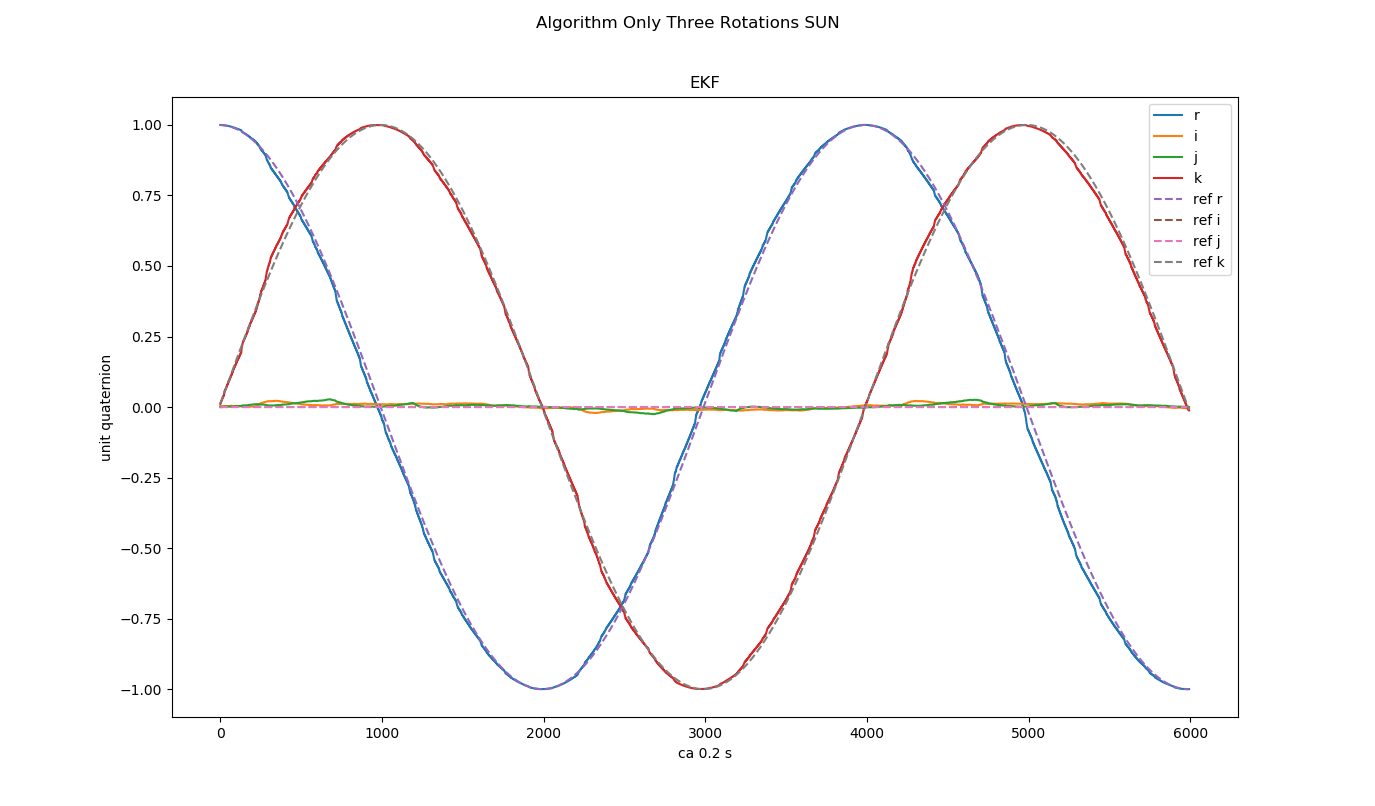
\includegraphics[width=1\columnwidth]{./Pictures/cdrRun3ThreeRotationsSun}
	\caption{Plot of recorded quaternion and reference quaternion for Algorithm only test using the PrintSat. Three rotations whit sun}
	\label{fig:cdr3RotSun}
\end{figure}               

\begin{figure}[tbp]
	\centering
	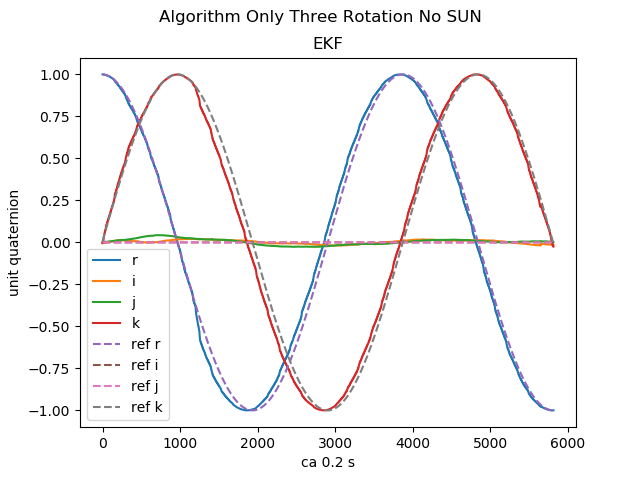
\includegraphics[width=1\columnwidth]{./Pictures/cdrRun3ThreeRotationsNoSun}
	\caption{Plot of recorded quaternion and reference quaternion for Algorithm only test using the PrintSat. Three rotations whit  no sun}
	\label{fig:cdr3RotNoSun}
\end{figure}

\subsection{PrintSat Outdoor Results}
When conducting the outdoor test there was no possibility of conducting tests whit rotations as there was problems getting the turntable to work whit batteries. A problem arises when there is no rotation. In \autoref{fig:OutdoorNoRotationSun} which is a test whit sun and no rotation it seems to be fine. The recorded quaternion is about [1 0 0 0] which is expected as the PrintSats body-fixed frame is aligned whit the lab frame. In \autoref{fig:OutdoorNoRotationNoSun} which is no sun and no rotation the EKF starts to struggle. From the results it seems like quaternions are converging towards the correct values, but the test is to short to say for sure what the quaternions are converging towards. Even if the quaternions are converging towards the right value it is way to slow. For the current implementation of the attitude controller this is not a  problem as it is a spinning controller, but one of the main reasons that the EKF is being implemented is to allow for the possibility to implement other types of controllers. One of this future controller could be a non spinning controller and the EKF should therefor be able to handle this scenario. Even if the problem does not affect the current design and is unlikely to come up in use it is a bug and before the root cause is discovered it is impossible to say what other side effects it might have.

\begin{figure}[tbp]
	\centering
	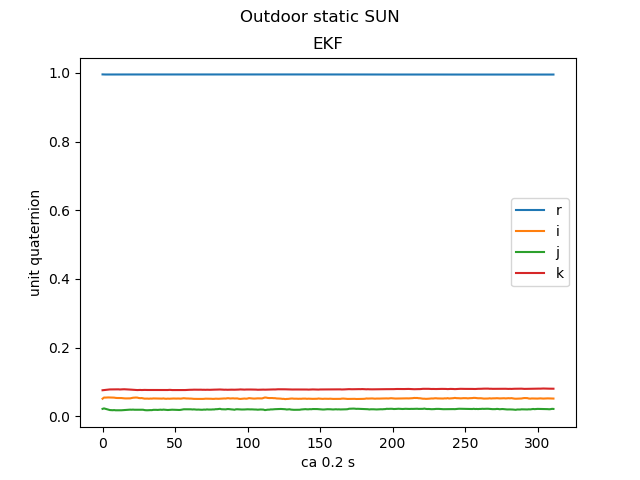
\includegraphics[width=0.6\columnwidth]{./Pictures/run3OutdoorStaticSUN}
	\caption{Plot of recorded quaternion quaternion for Outdoor test using the PrintSat. Static test whit sun}
	\label{fig:OutdoorNoRotationSun}
\end{figure}

\begin{figure}[tbp]
	\centering
	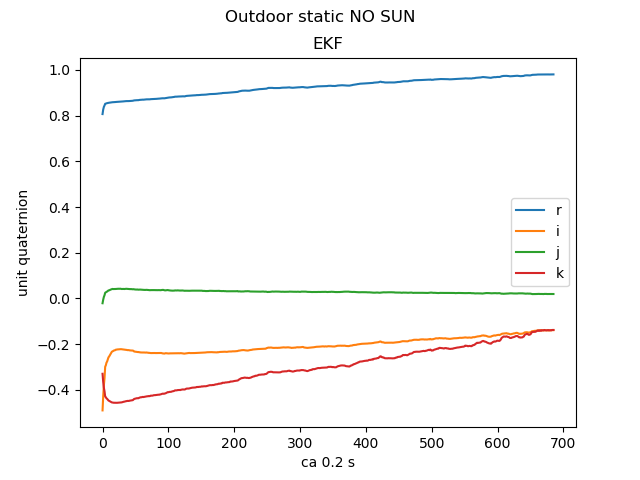
\includegraphics[width=0.6\columnwidth]{./Pictures/run3OutdoorStaticNOSUN}
	\caption{Plot of recorded quaternion for Outdoor test using the PrintSat. Static whit  no sun}
	\label{fig:OutdoorNoRotationNoSun}
\end{figure}         

Some effort have been put into trying to figure out why this happens. An initial theory was that it is due to the fact that the EKF is not initialized by the SVD and that it will converge to the right value give enough time. It is just so slow because the initial estimate is so far away from the correct estimate. The problem whit this theory is that the ADS seems to work when there is rotation and no sun. In this scenario there is also no SVD initialization, so it seems like the EKF works even whit out the SVD initialization. As a part of the future investigation a static Algorithm only test where conducted where the conditions where changed from sun to no sun before it was set back to sun. The results can be seen in \autoref{fig:cdrSunNoSunSun}. The results show that the quaternions stay constant even when there is sun if they have converged to the right values first. This at least indicates that the EKF does not diverge if the quaternions have already converge to the right value. For future investigation the problem have been recreated in simulations. This also indicates that the problem is a problem whit the algorithm it self and not the implementation on the satellite or any hardware related issues. 

\begin{figure}[tbp]
	\centering
	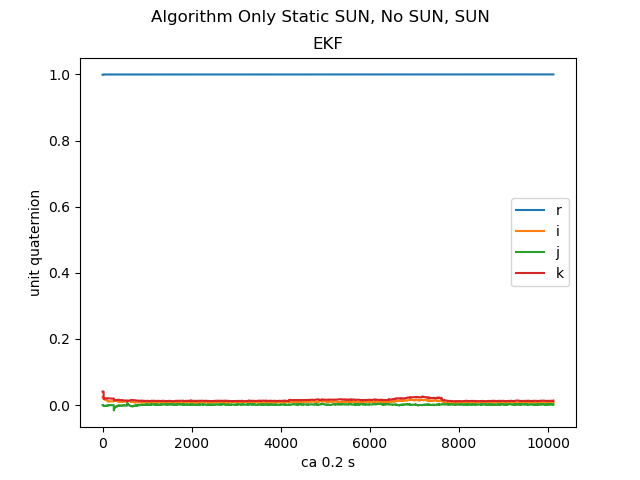
\includegraphics[width=0.6\columnwidth]{./Pictures/cdrRun1StaticSunEclipsSun}
	\caption{Plot of recorded quaternion for Algorithm only test test using the PrintSat. Static test where the condition are changed from sun to no sun and then back to sun. }
	\label{fig:cdrSunNoSunSun}
\end{figure} 

\subsection{PrintSat Reference Model Verification}
During the Outdoor test it is also possible to investigate how close the measurements are to there respective reference models. In \autoref{fig:magRef} the measured magnetometer data is plotted whit the reference magnetic vector from simulation and the one from reference vector calculated by the PrintSat. The simulated reference vector and the reference vector calculated by PrintSat are seemingly exactly the same, confirming that the reference vector calculated on the PrintSat is correct. There is some discrepancy between then measured vector and the reference vector, but overall it looks good. The main discrepancy is in the measurement of the z-axis. This also leads to a a difference between the lengths of the vectors. This error is not significant as when you normalize the vectors they become practically the same and the EKF uses the normalized vector. The error can also most likely be avoided by changing some of the parameters in the calibration procedure of the magnetometer resulting in an increase scaling of the z value to match the reference vector.           

\begin{figure}[tbp]
	\centering
	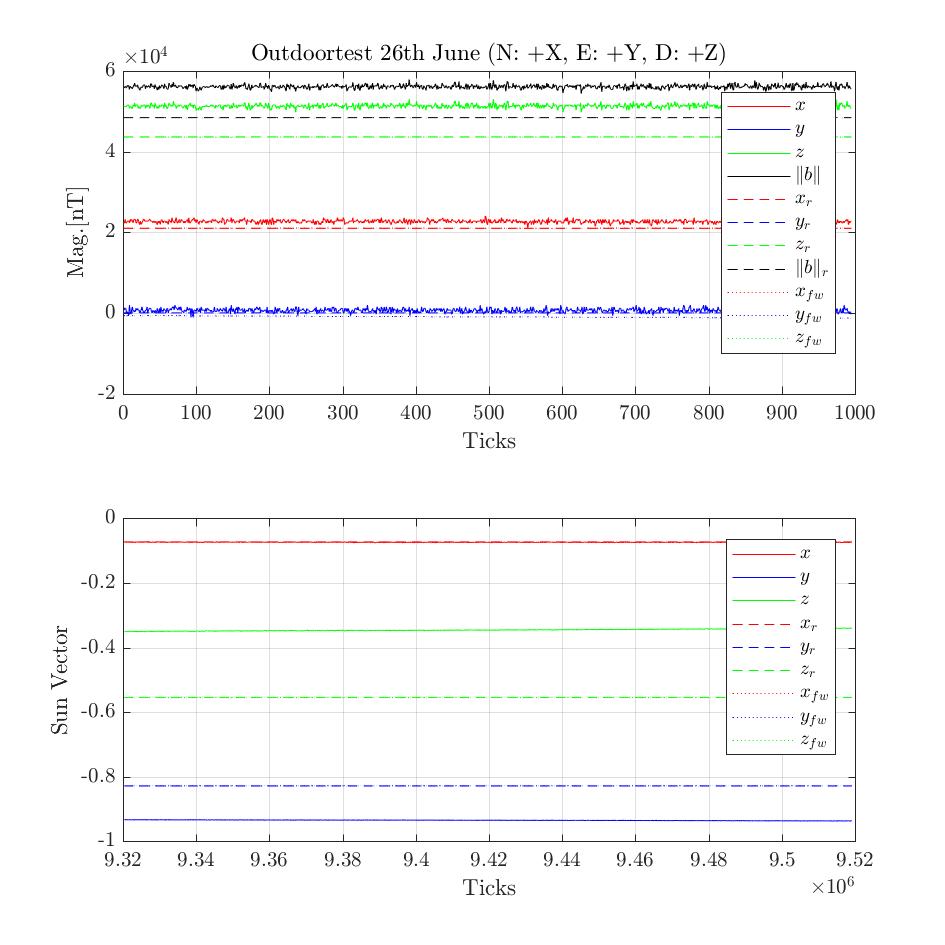
\includegraphics[width=0.8\columnwidth]{./Pictures/outdoor4}
	\caption{Plot of recorded magnetometer and sun sensor measurements plotted whit the simulated reference vectors and the reference vector calculated by the PrintSat. No lines subscript is sensor data, r subscript is simulated reference vector and subscript fw is reference vector from PrintSat}
	\label{fig:magRef}
\end{figure}

For the sun sensor the simulated and calculated reference vector are exactly the same meaning that the reference vector for the sun position is also correctly calculated on the PrintSat. The measured sun vector is quit far away from the reference vector. The reason for this is still not clear. All functionality test of the sun sensor indicates that they are working properly. A new method for calibrating the sun sensor where developed by another member of the ADCS team during this period. Despite using the new calibration method the results are still pore. A possible explanation could be that the error comes from the transformation of the measurements in sensor frame to the body-fixed frame. The transformation is assumed to be a \SI{90}{\degree} rotation around the axis of the body-fixed frame. This comes from the assumption that the side panels are parallel to the axis of the body-fixed frame. This assumption is not true on the PrintSat as the structure is not that rigged. The results also indicates that the EKF is capable to function even if the sun sensor measurements are not that good.                      

\section{Flight Model}
The test whit the FM where limited in scope and mostly to verify that the same behavior that is seen on the PrintSat can be seen on the FM. There results from two test shown in \autoref{fig:FMcdrTwoRotSun} and \autoref{fig:FMcdrTwoRotNoSun} show that the results are somewhat consistent whit the PrintSat. The overall trend in both is that ADS is preforming reasonably well and the estimated quaternions are able to follow the reference quaternions reasonably well. In \autoref{fig:FMcdrTwoRotSun} the preference is a lot worse than on the PrintSat equivalent test seen in \autoref{fig:cdr3RotSun}. There are this seemingly periodic shifts in the estimated quaternion that was not so viable on the PrintSat. This seems to come from spikes in the sun sensor measurements as you can see in the bottom plot of \autoref{fig:FMcdrTwoRotSun} there is a shift in the estimated quaternion when ever there are spikes in the sun sensor measurement. The spikes in the sun sensor measurements seem to come from when there is a switch in which sun sensor that is being used. The switching comes from  a new side panel facing the sun. The reason why the spikes in sun sensor measurements are only on the FM and not on the PrintSat is still under investigation, but the working theory is that the spikes comes from the environment. As the FM test was conducted in the integration room that is not completely dark while the PrintSat test where done in a complete dark room. The main reason environmental factors are consider the reason is that under all functional test of the FM sun sensors the sun sensors have preformed as expected and similar to the results to the sun sensor of the PrintSat.   

The one shift that can be seen in \autoref{fig:FMcdrTwoRotNoSun} also comes from when the natural light in the integration room was accepted as a valid sun sensor measurement and therefore used in the EKF cosing the shift. One thing that is interesting to note is that the quaternion does not converge back to the correct estimate but instead follows the reference quaternion whit a constant error.

\begin{figure}[tbp]
	\centering
	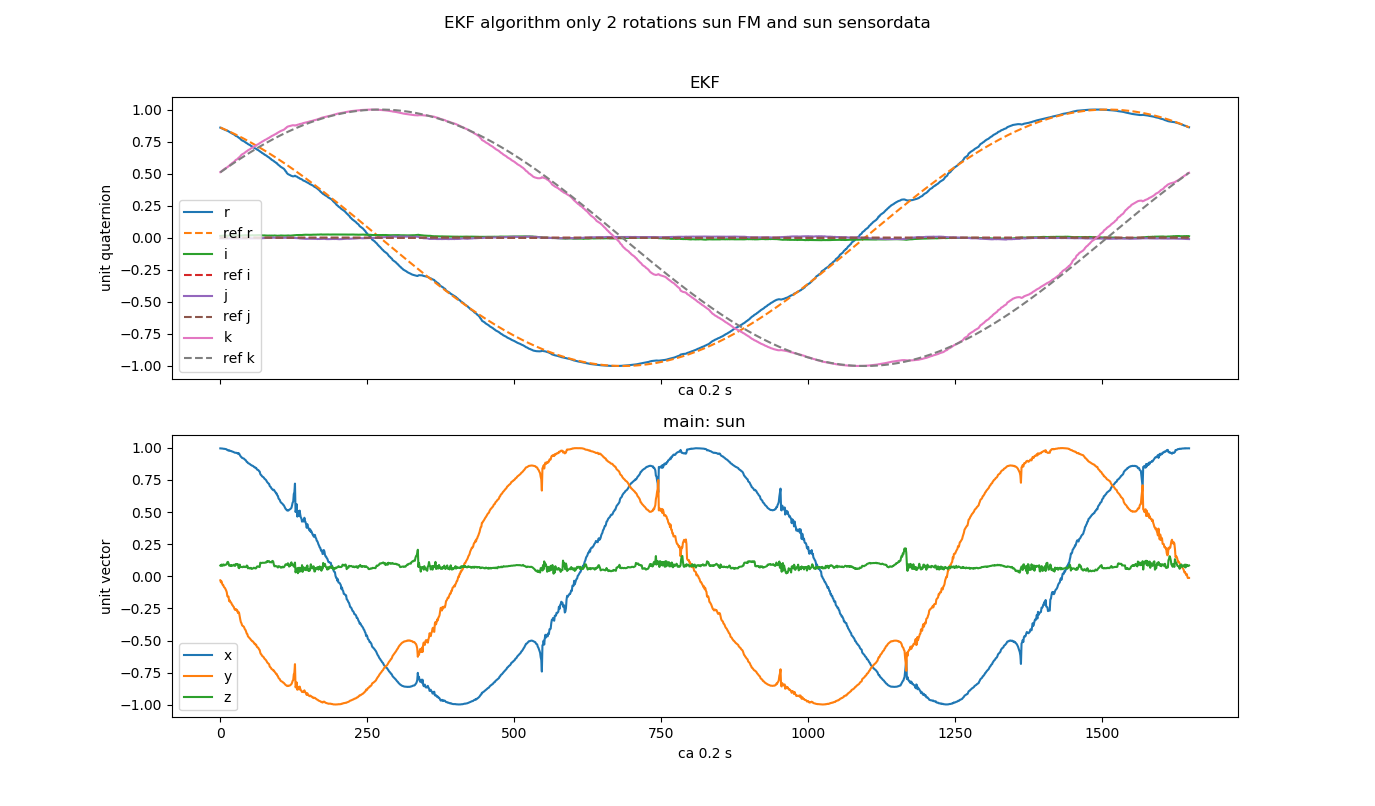
\includegraphics[width=1\columnwidth]{./Pictures/test1EKFandSUN}
	\caption{Plot of recorded quaternion for Algorithm only test test using the FM and the recorded sun sensor measurements. The FM is turned two time on the turntable.}
	\label{fig:FMcdrTwoRotSun}
\end{figure}

\begin{figure}[tbp]
	\centering
	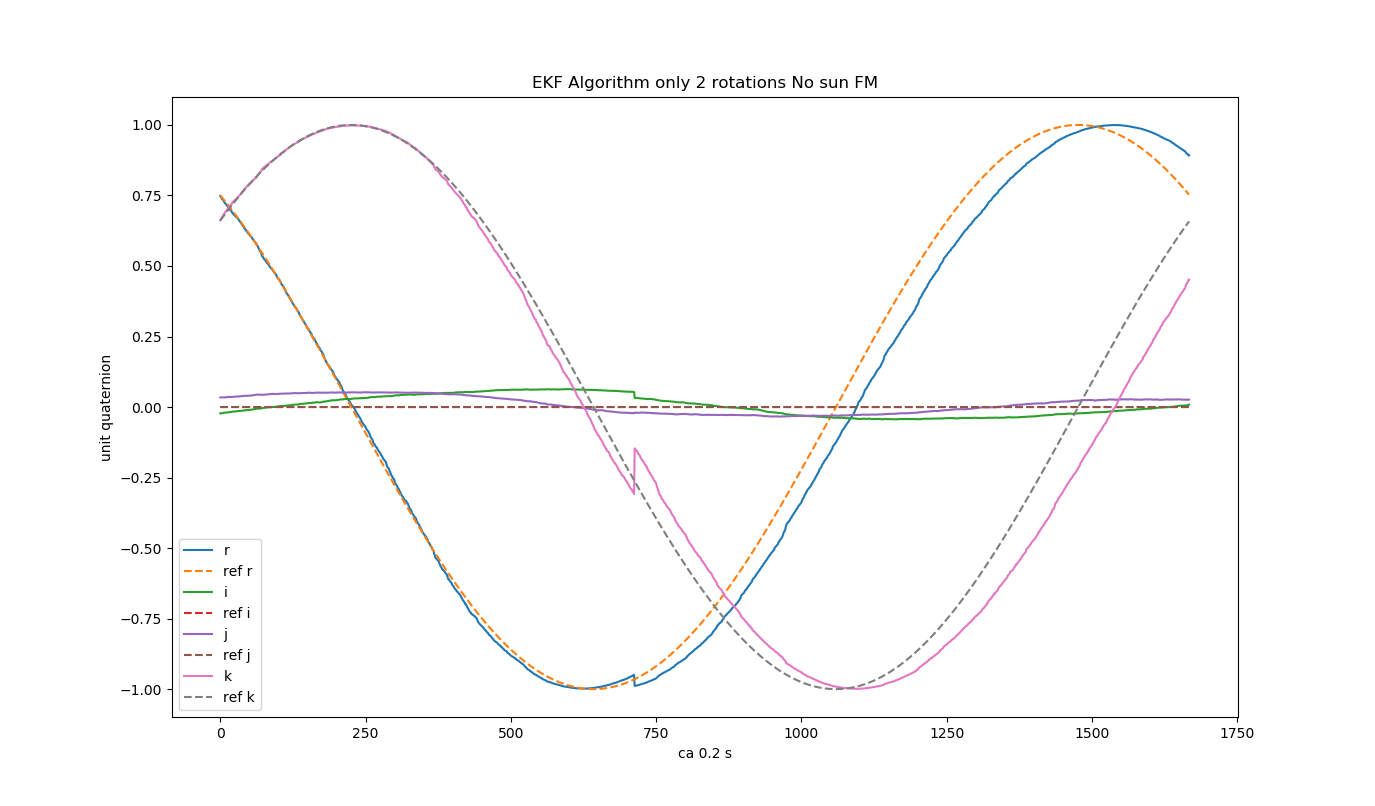
\includegraphics[width=1\columnwidth]{./Pictures/EKF_Algorithm_only_2_rotations_No_sun_FM}
	\caption{Plot of recorded quaternion for Algorithm only test using the FM. The FM is turned two times on the turntable.}
	\label{fig:FMcdrTwoRotNoSun}
\end{figure}   


